\documentclass{beamer}
\usepackage[T1]{fontenc}
\usepackage[utf8]{inputenc}
\usepackage[english]{babel}
\usepackage{verbatim}

%verbeek: pag 52 cap 3

% see https://tex.stackexchange.com/questions/68080/beamer-bibliography-icon/68084#68084 for reference
\usepackage[style=authoryear,dashed=false,backend=biber]{biblatex}
\usepackage{hyperref}

\setbeamertemplate{bibliography item}{%
	\ifboolexpr{ test {\ifentrytype{book}} or test {\ifentrytype{mvbook}}
		or test {\ifentrytype{collection}} or test {\ifentrytype{mvcollection}}
		or test {\ifentrytype{reference}} or test {\ifentrytype{mvreference}} }
	{\setbeamertemplate{bibliography item}[book]}
	{\ifentrytype{online}
		{\setbeamertemplate{bibliography item}[online]}
		{\setbeamertemplate{bibliography item}[article]}}%
	\usebeamertemplate{bibliography item}}

\defbibenvironment{bibliography}
{\list{}
	{\settowidth{\labelwidth}{\usebeamertemplate{bibliography item}}%
		\setlength{\leftmargin}{\labelwidth}%
		\setlength{\labelsep}{\biblabelsep}%
		\addtolength{\leftmargin}{\labelsep}%
		\setlength{\itemsep}{\bibitemsep}%
		\setlength{\parsep}{\bibparsep}}}
{\endlist}
{\item}

% general data
\title{Smart Home Ambient Intelligence: \\a new limit for our freedom?}
\subtitle{\vspace*{0.3cm}ethical concerns about voice assistants}
\author[Stefano Brandoli]{Stefano Brandoli}
\institute[PoliMi]{Politecnico di Milano}
\date{December 12, 2017}

%theme and aspect
\setbeamertemplate{navigation symbols}{}
\addbibresource{bibliography.bib}
%\usetheme{metropolis}

\begin{document}

% frame
\begin{frame}
\maketitle
\end{frame}

% frame
\begin{frame}
\begin{center}\vspace*{-0.5cm}Smart Home Ambient Intelligence: a new limit for our freedom?
ethical concerns about voice assistants
\end{center}
\frametitle{Presentation Outline}
\tableofcontents
\end{frame}

\section{Introduction}

% interleave
\begin{frame}
\begin{center}
	\usebeamerfont*{frametitle}
	\usebeamercolor[fg]{frametitle} Introduction
\end{center}
\end{frame}

\subsection{Technological Mediation}
% frame
\begin{frame}[fragile]
\frametitle{Technological Mediation}
\begin{quote}While fulfilling their function, technologies do much more: they \textbf{give shape to what we do} and how we experience the world. 
	And in doing so they \textbf{contribute actively} to the ways we live our lives (\cite{verbeek2011moralizing})
\end{quote}

\begin{itemize}
	\item Technologies are not \textbf{neutral intermediaries}
	%give shape to what we do and how we experience the world
	\item Technologies play an \textbf{actively mediating role} 
	%in the relationship between human beings and reality. No mute and passive objects
	\item Artifacts are \textbf{bearers of morality} (\cite{latour1992})
	%as they help people to make all kinds of moral decisions
	\item Morality is a matter of \textbf{human-technology associations}

\begin{comment}
%	not an exclusively human affair, since it requires intentions and freedom.
%	vs rigid separation of humans vs non humans in Latour words.
%	The only adequate way to understand it is in terms of its hybrid character.
%	it cannot be reduced to either an object or a subject but needs tounderstood in terms of their mutual relations. 
%moral action cannot be understood here
in terms of a radical separation of a human moral agent, on the one hand,
acting in a world of mute material objects on the other. 
\end{comment}

\end{itemize}

\begin{itemize}
	\item Two perspectives of mediation:
	\begin{itemize}
		\item Perception
		\item \textbf{Action}: I will focus on \textbf{human freedom}
		%Its central question is how human beings act in their world and shape their existence.
	\end{itemize}
\end{itemize}

\end{frame}

\subsection{Definitions}
% frame
\begin{frame}[allowframebreaks]
\frametitle{Definitions}
{\small 	\begin{block}{Ambient Intelligence}
		\begin{quote}
			\textbf{Ambient Intelligence} is an approach that combines two major technologies: Ubiquitous Computing and Intelligent User Interfaces (\cite{brey2005freedom})
		\end{quote}
	\end{block}

	\begin{block}{Voice Assistant}
		\begin{quote}
			A \textbf{voice assistant} is a digital assistant that uses voice recognition, natural language processing and speech synthesis to provide aid to users through phones and voice recognition applications (\cite{whatis})
		\end{quote}
	\end{block}
	\framebreak
	\begin{block}{Freedom}
		\begin{quote}
			\textbf{Ambient Intelligence} is an approach that combines two major technologies: Ubiquitous Computing and Intelligent User Interfaces. 
		\end{quote}
	\end{block}
}
\end{frame}

\section{Case Study: Google Home - Google Assistant Actions}

% interleave
\begin{frame}
\begin{center} 
	\usebeamerfont*{frametitle}
	\usebeamercolor[fg]{frametitle} Case Study: Google Home - Google Assistant Actions
\end{center}

\begin{figure}
	\centering
	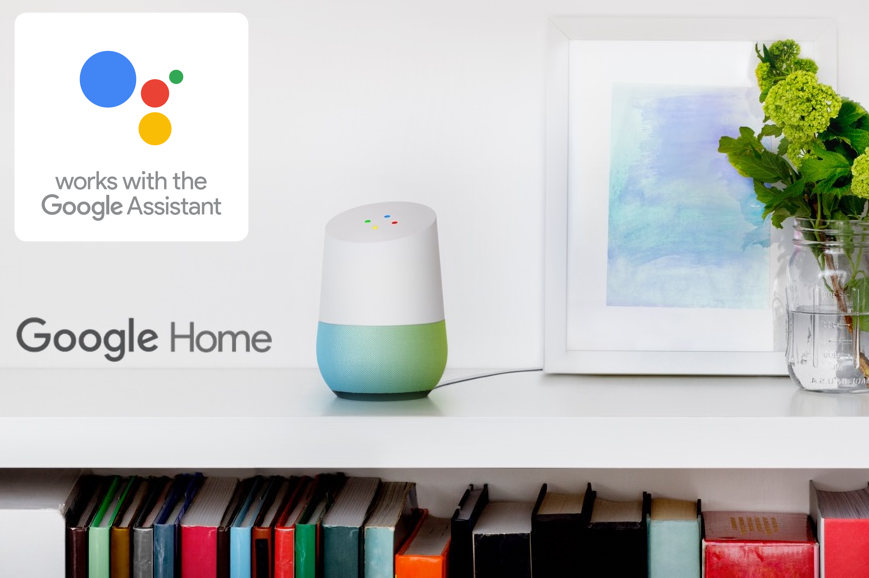
\includegraphics[width=0.95\linewidth]{images/Google-Home1}
	\label{fig:maxresdefault}
\end{figure}

\end{frame}

% frame
\begin{frame}
\frametitle{Google Assistant Actions}
\end{frame}

\subsection{Technological mediations further limiting our freedom}
% frame
\begin{frame}
\frametitle{Script}
\end{frame}

% frame
\begin{frame}
\frametitle{Invitation/Inhibition structure}
\end{frame}

% frame
\begin{frame}
\frametitle{Behaviour Steering}
\end{frame}

\subsection{Ethical concerns arising from loss of freedom}

% frame
\begin{frame}
	\frametitle{Moral laziness}
\end{frame}

% frame
\begin{frame}
	\frametitle{Technocracy}
\end{frame}

% frame
\begin{frame}
	\frametitle{Technological mediation? }
\end{frame}

% frame
\begin{frame}
	\frametitle{Moral responsibility of designers}
\end{frame}

\section{Possible Remedies}
% interleave
\begin{frame}
\begin{center} 
	\usebeamerfont*{frametitle}
	\usebeamercolor[fg]{frametitle} Possible Remedies
\end{center}
\end{frame}

% frame
\begin{frame}
\frametitle{Possible Remedies}
\end{frame}

\section{Conclusions}
% interleave
\begin{frame}
\begin{center} 
	\usebeamerfont*{frametitle}
	\usebeamercolor[fg]{frametitle} Conclusions
\end{center}
\end{frame}

%frame
\begin{frame}
\frametitle{Conclusions}
\end{frame}

% bibliography frame,see https://tex.stackexchange.com/questions/68080/beamer-bibliography-icon/68084#68084 for reference
\nocite{*}
\begin{frame}[noframenumbering,plain,allowframebreaks]{Bibliography}
\renewcommand*{\bibfont}{\footnotesize}
\printbibliography
\end{frame}

\end{document}